\documentclass[11pt, titlepage]{article}

\usepackage[margin=1in]{geometry}
\usepackage[strict]{changepage}
\usepackage{float}
\usepackage{fancyhdr}
\usepackage{mhchem}
\usepackage{siunitx}
\usepackage{wrapfig, booktabs}
\usepackage{enumitem}
\usepackage{caption}
\usepackage{commath}
\usepackage{amsmath}
\usepackage[hang]{footmisc}
\usepackage{multicol}
\usepackage{amsfonts}
\usepackage{mathrsfs}
\usepackage{mathtools}
\usepackage{tikz}

% my imports
\usepackage[most]{tcolorbox}
\usepackage{hyperref}
\hypersetup{
    colorlinks,
    citecolor=black,
    filecolor=black,
    linkcolor=black,
    urlcolor=black
}

\newcommand{\experimentDate}{\today}
\newcommand{\className}{CSE 371}
\newcommand{\assignmentname}{Lab 6}
\author{Donovan Clay (ID: 2276005), Cameron Jennings (ID: 2029631)}
\newcommand{\authorLastName}{Clay, Jennings}
\title{\assignmentname}

\date{\parbox{\linewidth}{\centering
\experimentDate
  \endgraf\bigskip
  \className\
}}

\pagestyle{fancy}
\fancyhf{}
\setlength{\headheight}{13.59999pt}
\rhead{\authorLastName\ \thepage}
% \lhead{\experimentShortName}
\lhead{\hyperref[beginning]{\assignmentname}}
\cfoot{\className\ -- \assignmentname}

\usepackage{color}
\usepackage{sectsty}

\definecolor{WordSectionBlue}{RGB}{30, 90, 147}

\allsectionsfont{\color{WordSectionBlue}}

\tcbuselibrary{breakable}

\begin{document}
	\maketitle
 
    \setcounter{tocdepth}{2}
    \begin{center}
        \tableofcontents\label{beginning}
    \end{center}
    \newpage
    
    \section{Design Procedure}
    In this lab, we decided to build Space Invaders as we were tasked to design our own project. The system implements the provided N8 controller and VGA display driver modules. The N8 controller's joystick controls the movement of the player and the buttons register the firing of the lasers. The purpose of the game is to fire the laser to kill all 20 of the aliens on the display. Once this is done, the game is over. There are additional modules and systems implemented in the program to control, update, and simulate the player, laser, and aliens on the VGA display. There is a global reset switch on SW[0] to start or restart the game.
        
        \subsection{Display RAM Module}
            In this lab, the VGA driver we are provided ``gives'' a xy-coordinate on the screen and asks for the color that the pixel should be. So we thought the easiest way to implement the display would be to use a 2-port RAM to store the color of every pixel on the screen. The VGA driver is free to read from the RAM whenever it wants and from wherever it wants. The other read/write port is for updating the data whenever the game dictates that the screen should look different. Since colors are 24 bit numbers in this implementation, it was far too much memory to store the full 24bit encoding of every pixel. So, we figured we could just ``which color'' the pixel should be. For example, store 0 for black, 1 for red, 2 for blue. This meant we could reduce the width of each address enormously. So the RAM only stores 4 bits at each address.

        \subsection{Color Converter Module}
            With the display RAM module only storing ``which color'' and not the actual encoding of the color, we needed a decoder so the VGA driver could be supplied the correct information about the color of pixels. So this color converter module is pretty much a 16 to 1 MUX, with many of the inputs undefined because we only ended up using 5 colors. 

        \subsection{Aliens Alive RAM Module}
            The game must hold state of which aliens are alive and which are dead. We decided to use a RAM to hold this information. The RAM holds 20 1-bit words: 0 for dead, 1 for alive.

        \subsection{Player Location Module}
            This module holds the XY coordinate of the player. When the user presses left on the controller, the x coordinate decreases and when the user presses right on the controller, the y coordinate increases. The module also constrains the location of the player to walls of the screen. Meaning if you hold left, you will eventually hit an invisible wall on the left side of the screen and the spaceship won't move anymore to the left.

        \subsection{Alien Group Location Module}
            This module holds the XY coordinate of the group of aliens. Since all the aliens move as a group, we only need to know the location of the group to know the location of each alien. The group of aliens move left and right across the screen and when they reach the left or right side of the screen they move a little bit closer to the player's side of the screen.

        \subsection{Drawing State Machine Module}
            \begin{figure}[H]
                \centering
                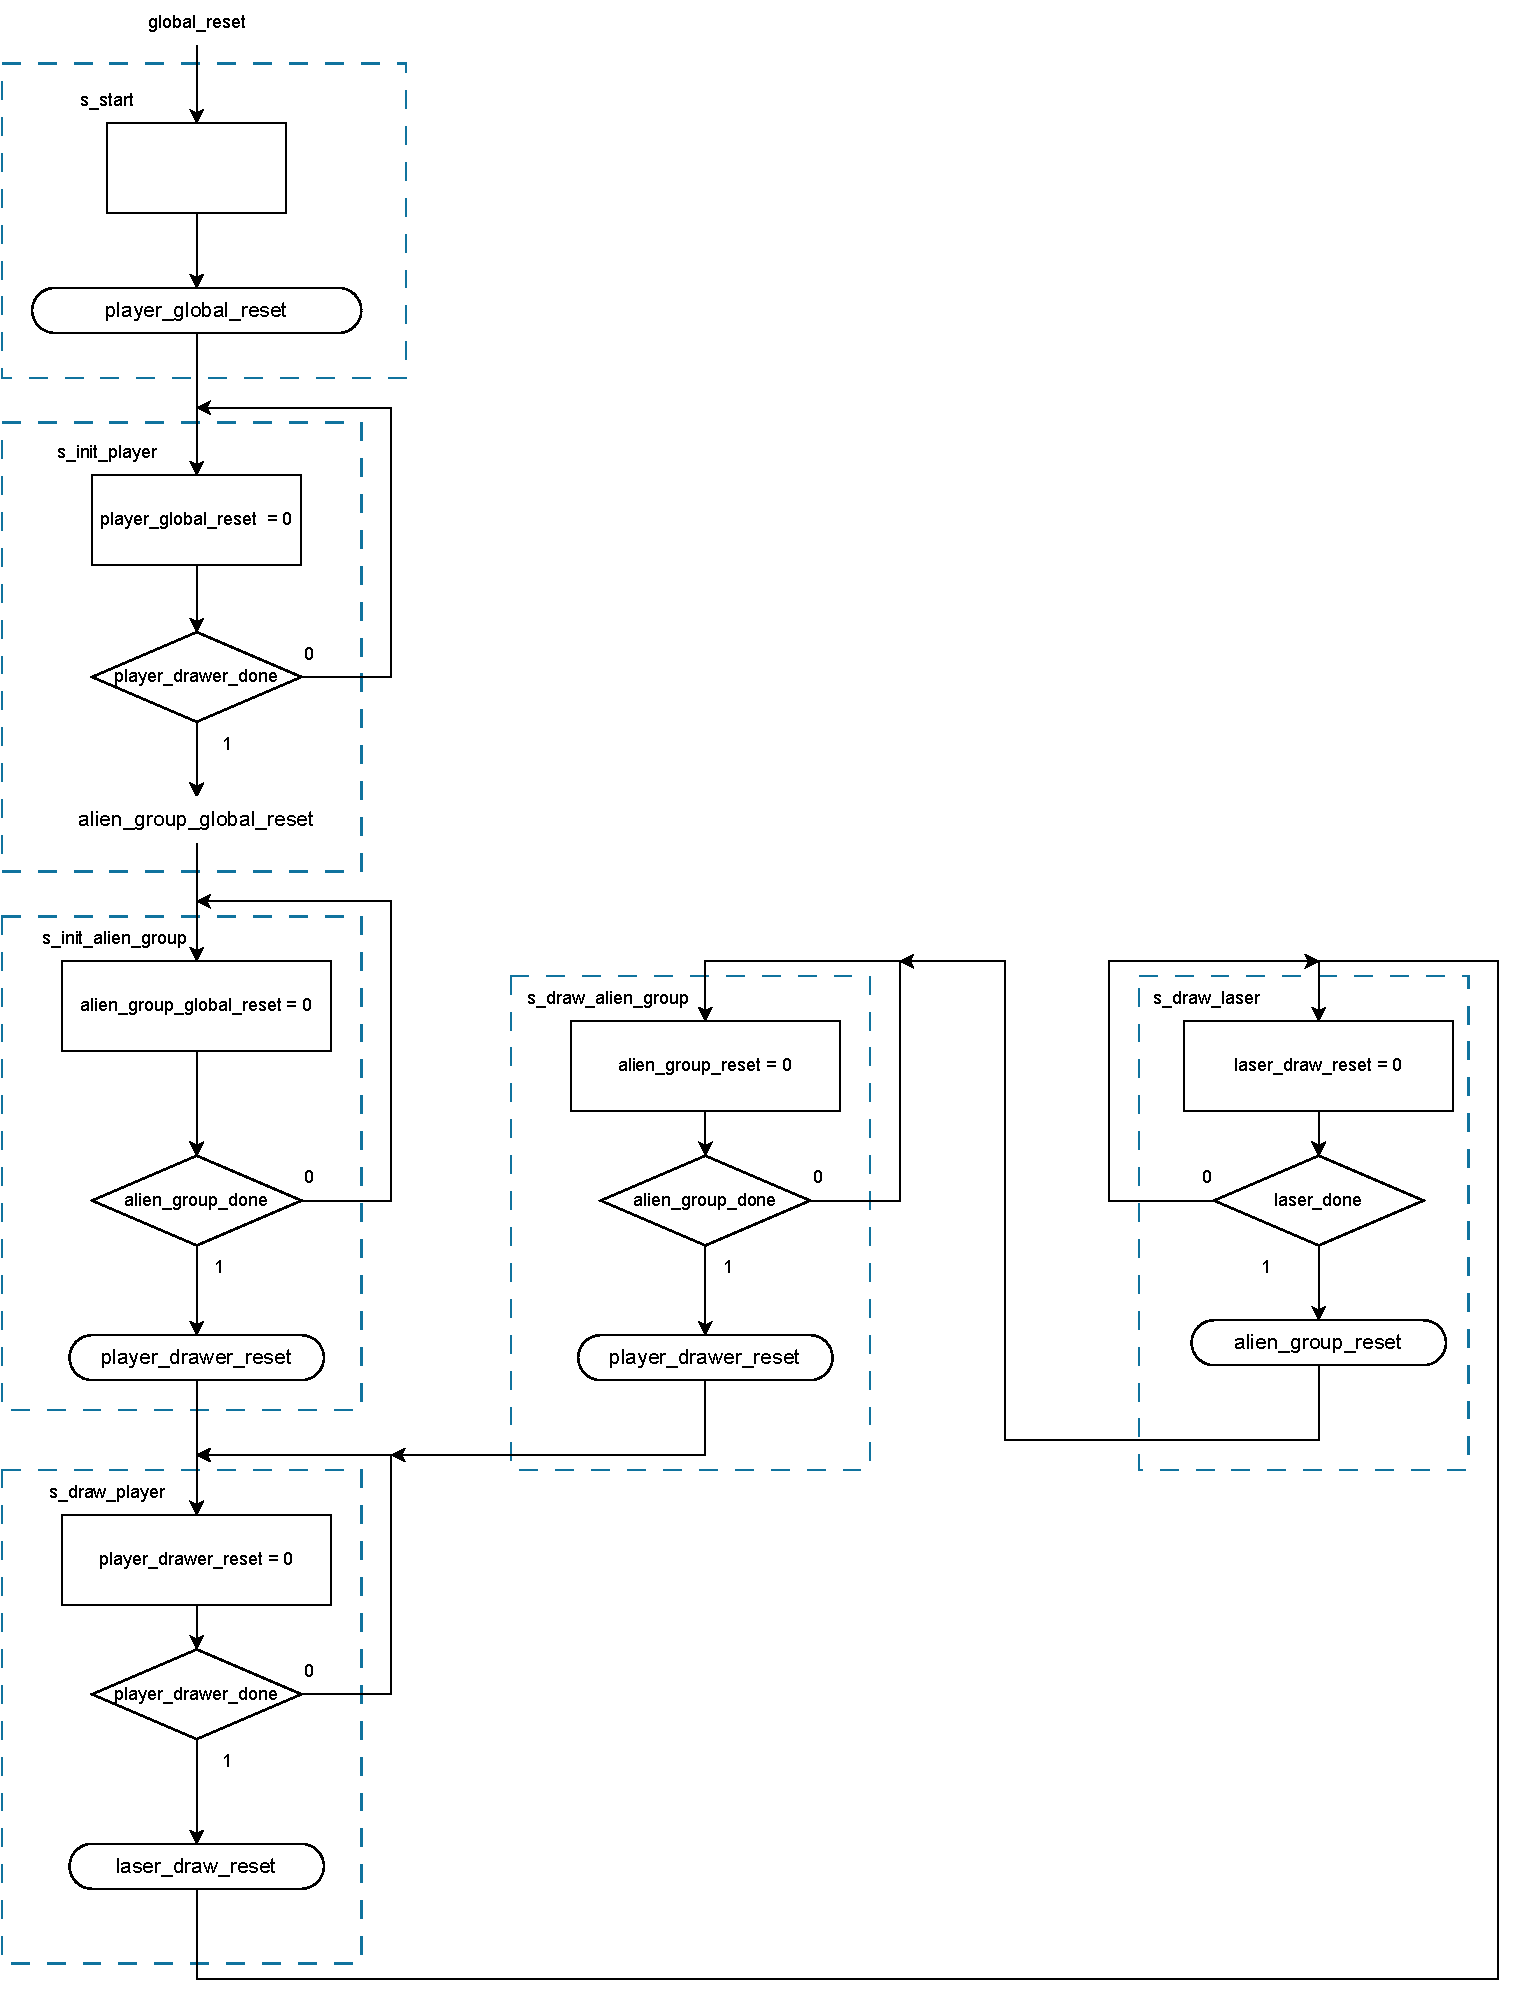
\includegraphics[scale = 0.59]{Images/Drawing State Machine ASM.pdf}
                \caption{Drawing State Machine ASM chart}
            \end{figure}
            The drawing state machine is responsible for updating the players, aliens, and lasers on the VGA display based on the state of the game. The game first begins with a global reset switch that syncs the system to the start state and resets to the beginning conditions. The start stage only lasts one clock cycle as only a brief moment is needed to reset the system before switching to the initialized player stage. Whether the game is just beginning or a new game is started from an old one, the player on the VGA display must be reset to its default location. After this, the player is drawn for the new game. This stage lasts for as long as it takes for the system to draw the new player. The next stage is similar to before but now the system must reset, initialize, and draw the aliens. The state of whether the alien is alive or not is stored in a RAM file, so the RAM must be reset so the program knows to draw all 20 of the aliens. The initialized aliens stage takes as long as the system needs to draw all the aliens before moving on to the next stages in the system.
            The starting conditions of the system are now done and the game must be updated to simulate the playing experience. The N8 controller controls the movement of the player, it decides whether the player moves left/right, or if it shoots the laser. Based on the joystick inputs from the controller driver in the system, the location of the player must be updated. The old player location is erased from the VGA display and then drawn again to simulate movement. Once this is completed, the system moves onto the draw laser stage, which checks the laser button on the N8 controller to either draw another laser or update the location of another laser to simulate a moving blast. The laser system is explained in more depth in the next section. Once ll the new location of the laser is updated, the drawing state machine moves onto its final task, drawing the updated alien location. The RAM file must be checked to ensure the state of the alive aliens that must be drawn in the next update. Next, the location of all the aliens are updated. The aliens are restricted to only moving right or left until they hit a certain bound and must switch direction. Once, the state of the alive aliens is checked and all their locations are updated, the old copies must be erased and the new ones must be drawn. Again, the stage takes as long as the system needs to update and draw all the aliens. This is the last state in the machine before it transitions back to the player drawer stage so the cycle can continue. The moving parts of the game are the player, the aliens, and the lasers. Therefore the system must continuously cycle through updating and drawing them to simulate the movement of the game. The game only ends once the global reset key is switched or there are no more aliens in play.
        
        \subsection{Alien Group Drawer Module}
            \begin{figure}[H]
                \centering
                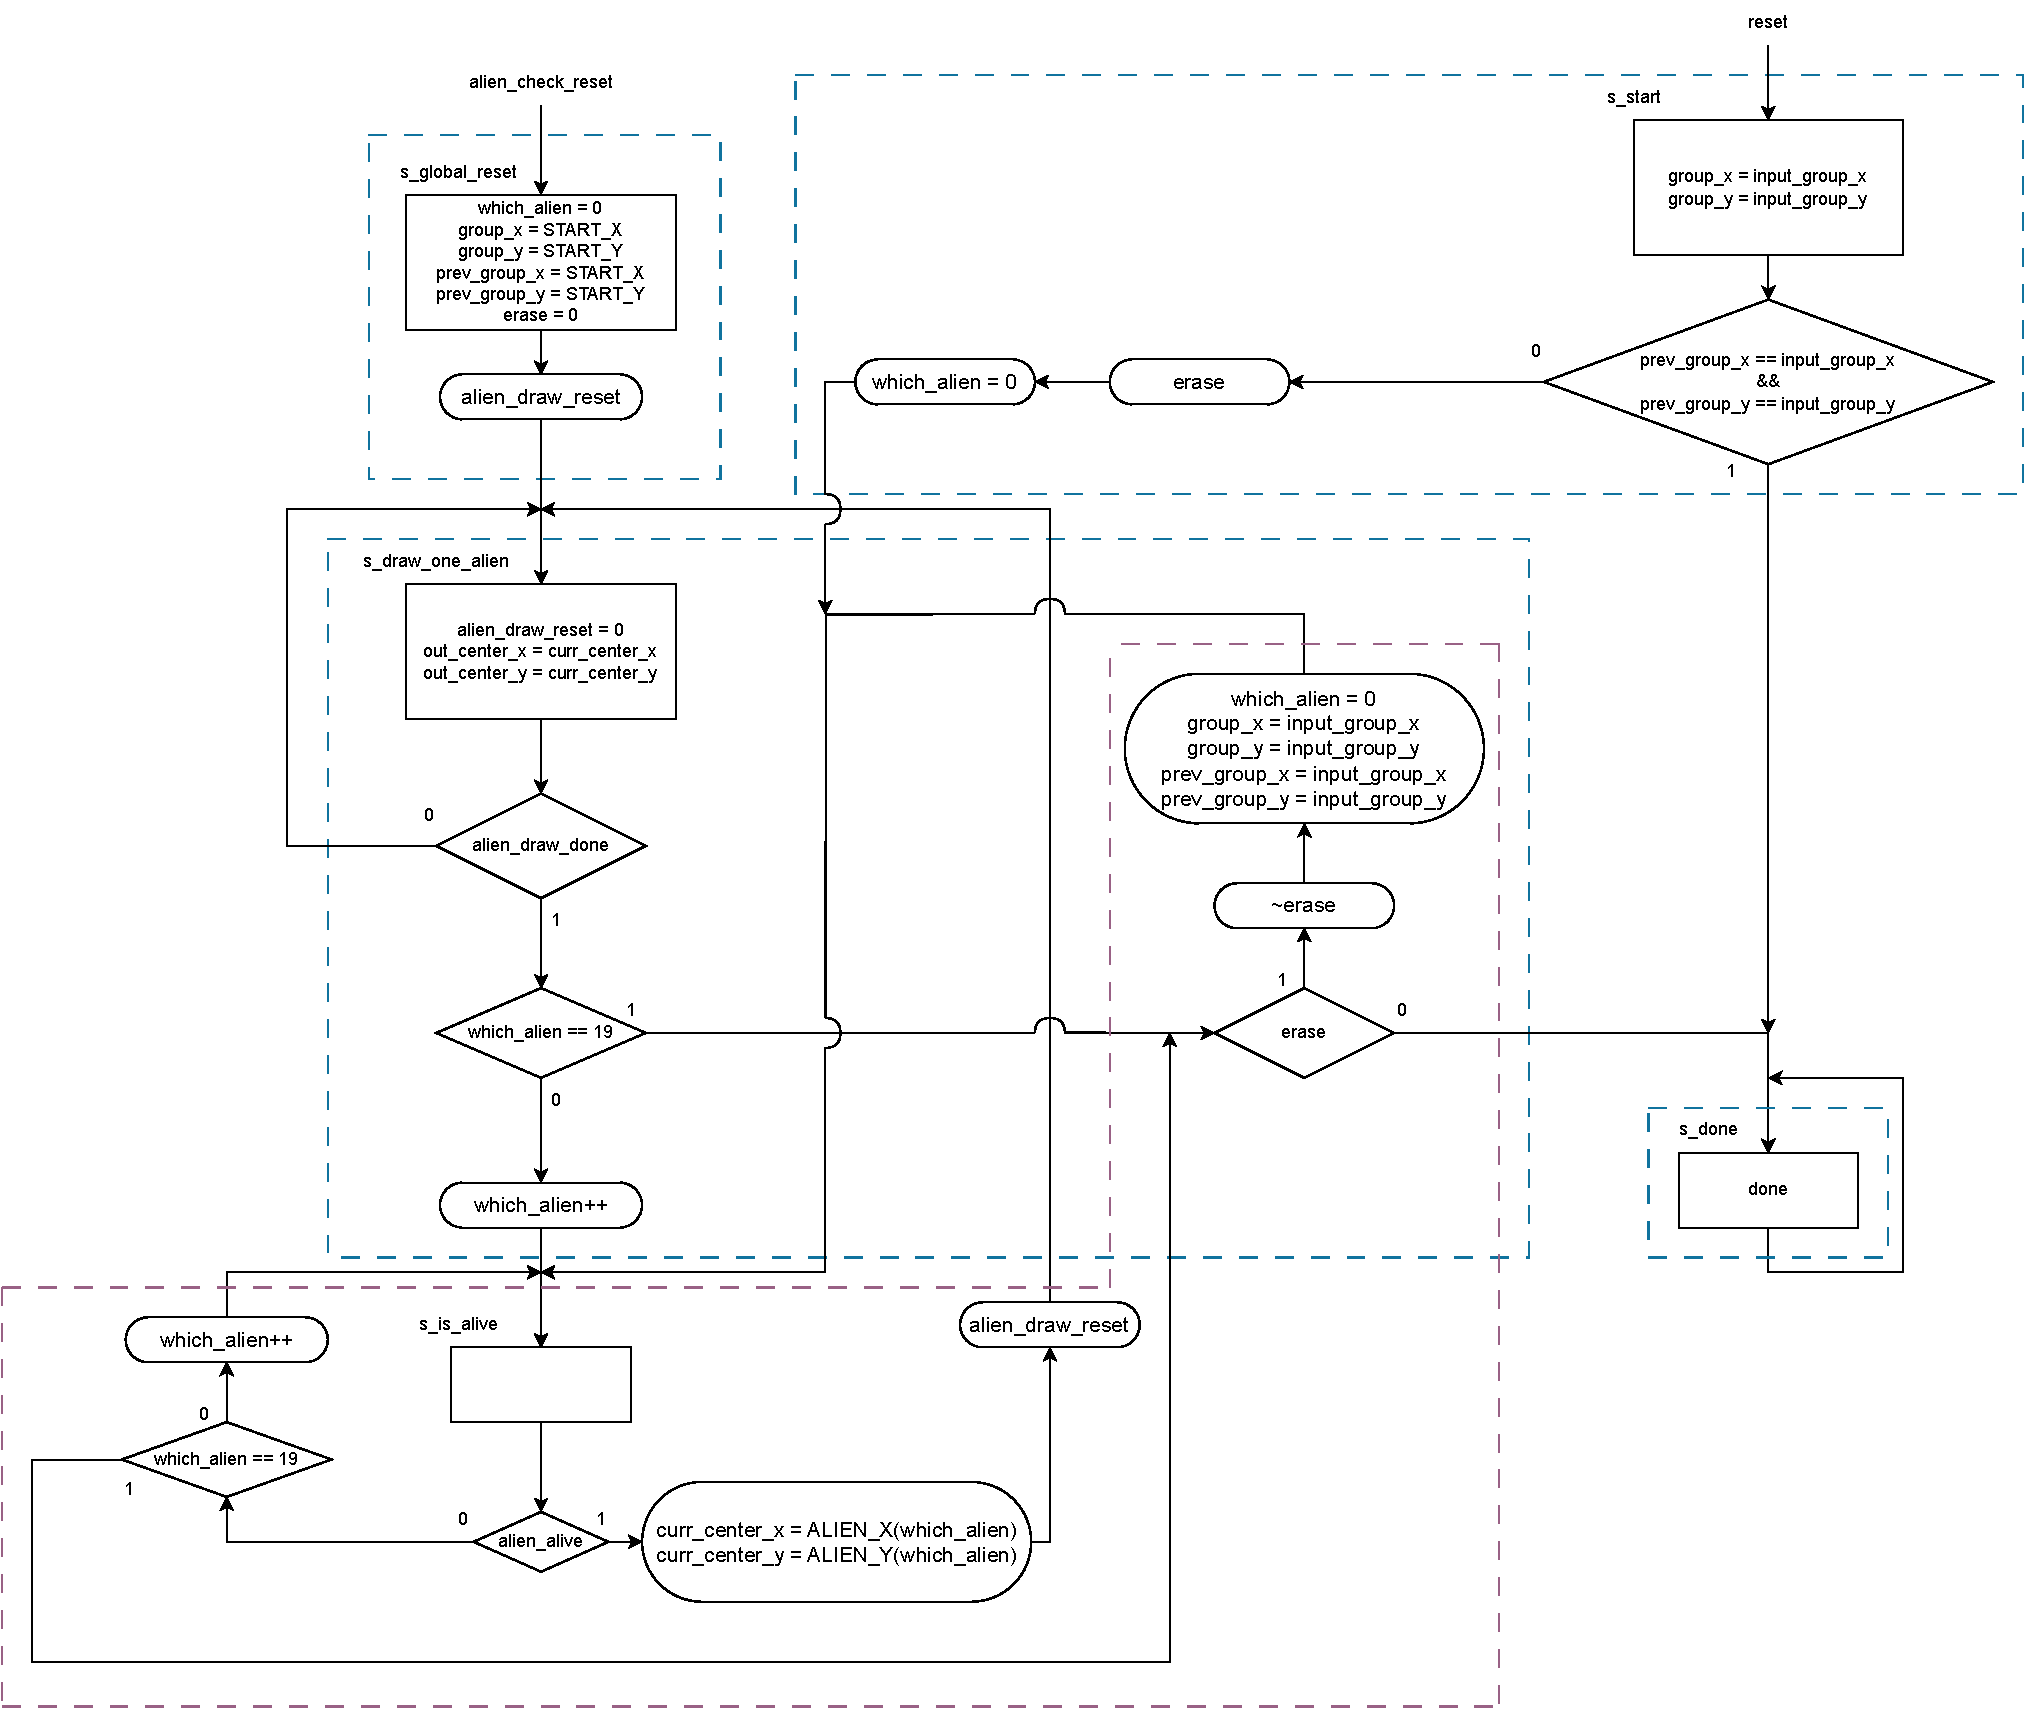
\includegraphics[scale = 0.45]{Images/Alien Group Drawer.pdf}
                \caption{Alien Group Drawer ASM chart}
            \end{figure}
            There is a state machine responsible for tracking and updating the values of all the aliens. The alien group drawer can start from a reset which resets all aliens and location back to the default values. Otherwise, the system is entered on a system restart and put in the start stage. In this stage, the location of the next cycle of aliens is passed as input into the system. The system compares if the previous value is equal to the expected. If so, then the machine entering the done stage exits. If the value of the alien locations has to be updated then the erase signal is turned high and the first alien is checked in the is alive state. If the alien is not alive, then the system checks if the algorithm has reached the last alien, again if not then the alien is increased and the search to find and alive alien countries by cycling through this stage. If the alien is alive, then the alien draw stage is entered. The location of this alien is updated in the alien drawer and the system stalls in the draw one alien stage until the other system is done. Once the system is done, then the number of alien is checked to see if it is the last alien again. If it is then there must be a final check of all the aliens before the system transitions to the done stage and terminates. In the case that it is not the last alien after updating, then the system switches to the is alive stage to find the next alive alien to update.

        \subsection{Alien Drawer Module}
            \begin{figure}[H]
                \centering
                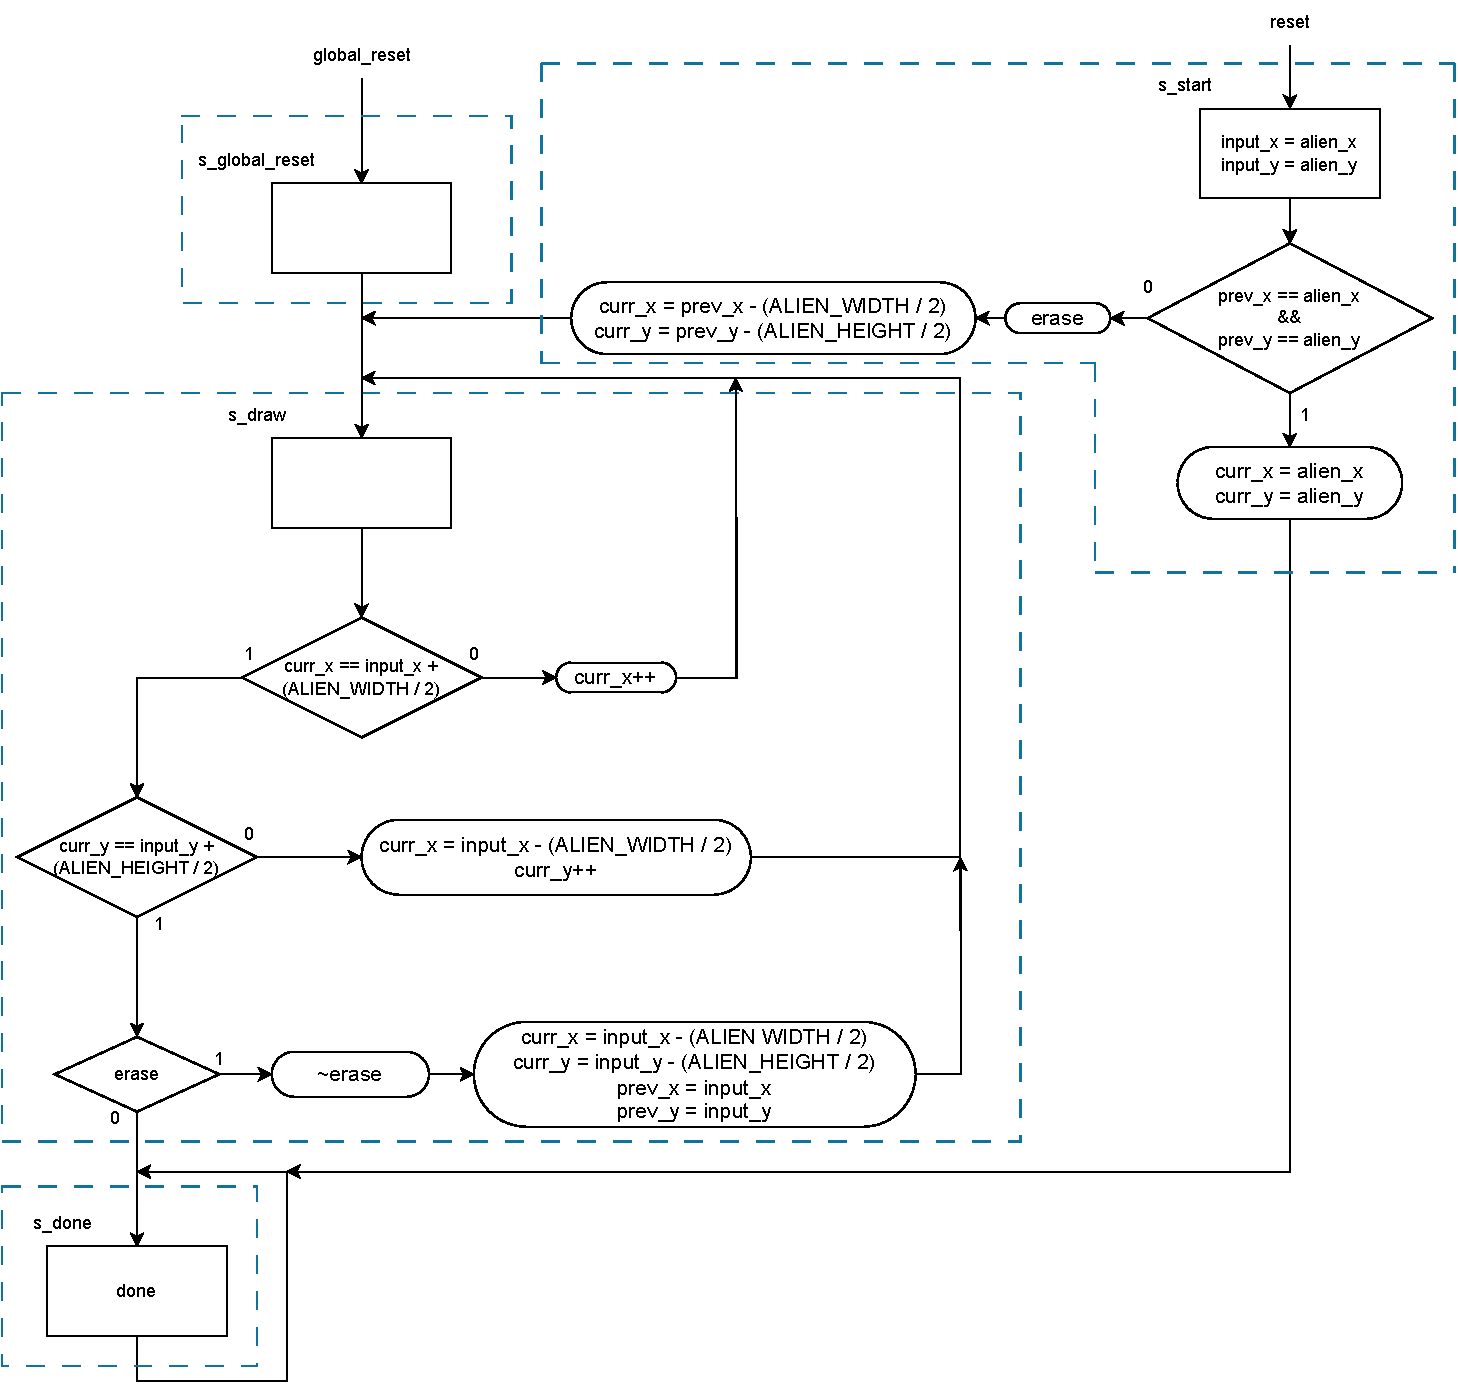
\includegraphics[scale = 0.57]{Images/Alien Drawer.pdf}
                \caption{Alien Drawer ASM chart}
            \end{figure}
            The alien drawer begins with a reset into the start state that sets the values of the alien location as input. If the previous alien value is equal to the alien values passed, then the current values are set accordingly and the next state of the machine is done. If the values of the aliens do not coincide with the previous values, then they must be redrawn so the erase signal is set high and then current values are set to alterations of the previous values before entering the draw stage. The draw stage can also be entered from a global reset which resets all values back to default. The draw stage continues to iterate until the current location of the alien is equal to that of the input. Once the x and y values are equal to the expected value, the erase signal is set low and the new location of the alien can be output and drawn onto the VGA display. The state of the machine then changes to done and exits.

        \subsection{Alien Check Module}
            \begin{figure}[H]
                \centering
                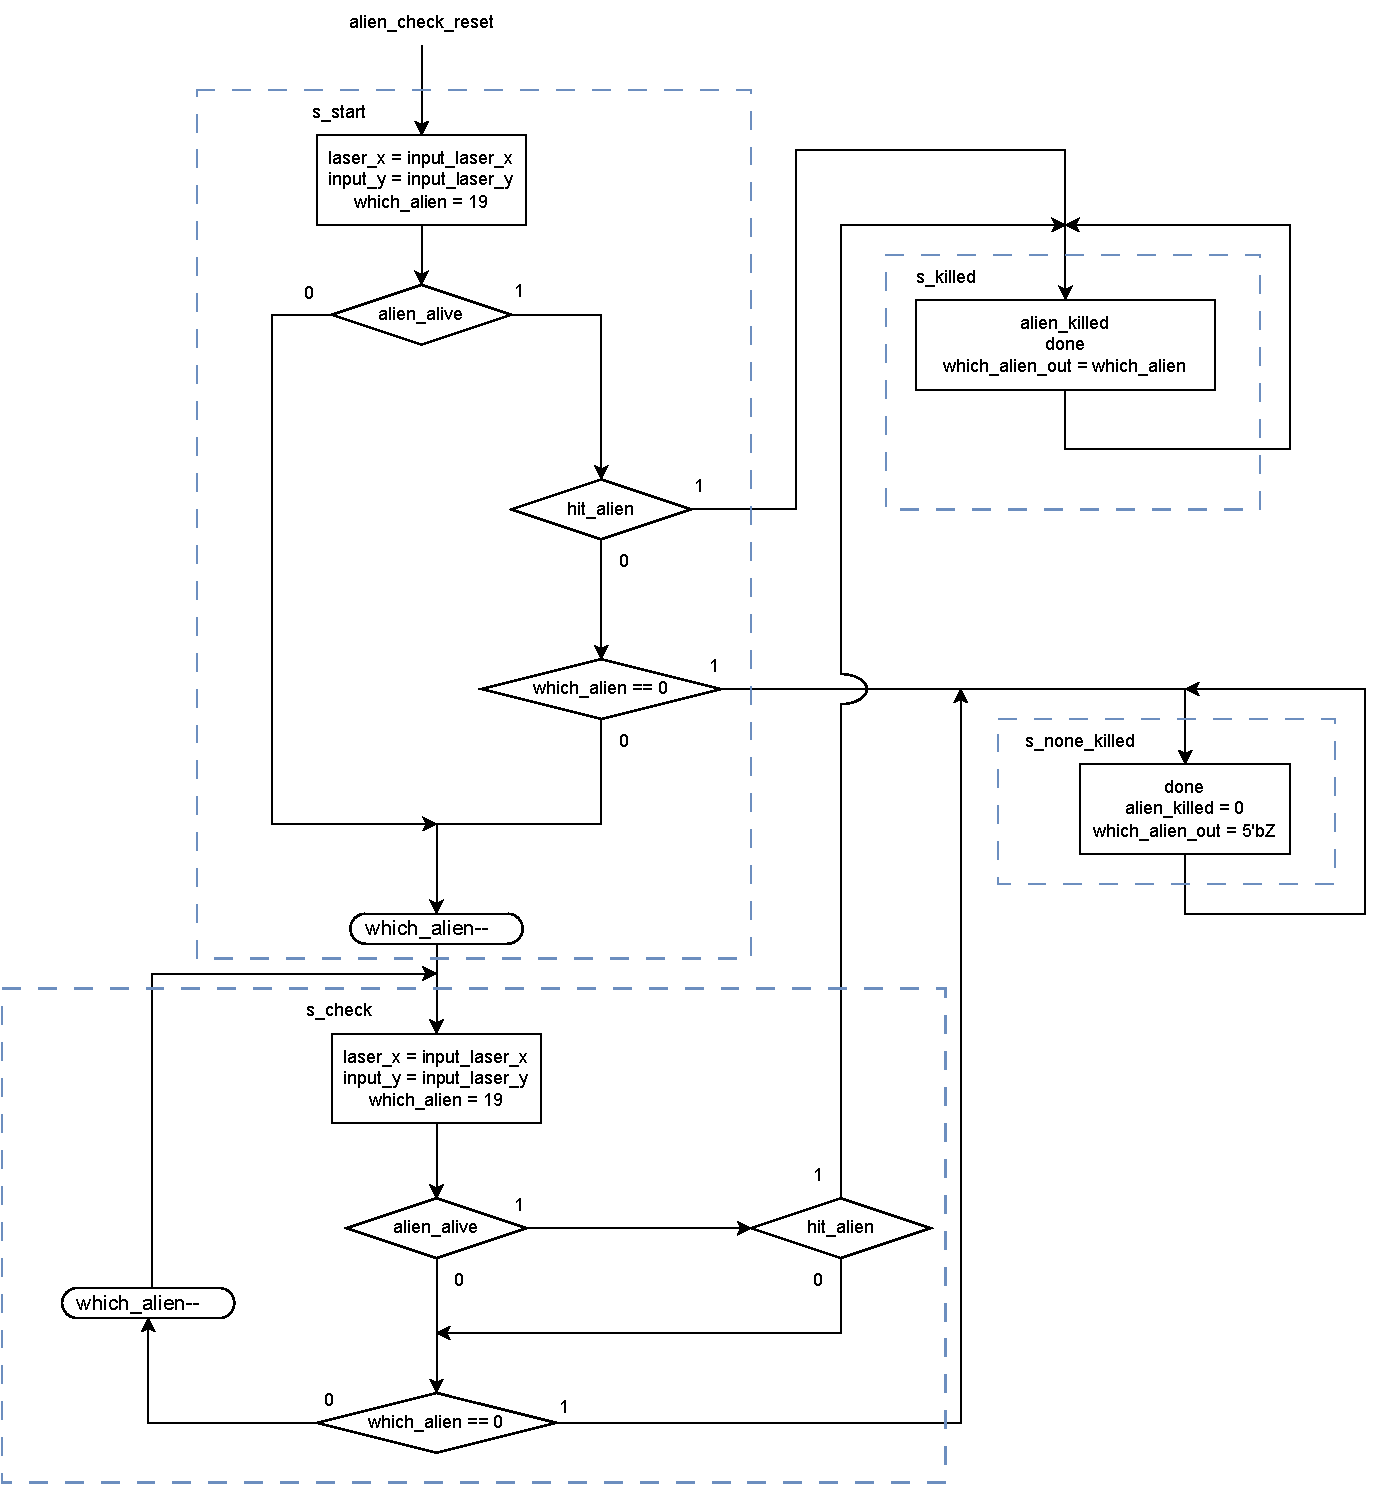
\includegraphics[scale = 0.57]{Images/Alien Check ASM.pdf}
                \caption{Alien Check ASM chart}
            \end{figure}
            The laser drawer uses an alien check state machine to determine whether a laser hit an alien or not. On reset, the system is entered in the start stage that takes the laser location x and y and resets the value of the alien to 19. The system then checks if the alien, number 19, is alive. If so then it determines if the alien is hit. Considering only one alien can be hit by one laser, once an alien is determined to be hit, the system transitions to the killed stage and the alien in question is output so the system can be updated. If that alien is not hit, then it switches to the next alien to check to see if the laser hit them or not.The system then repeats the process with the next alien. If all aliens are checked and none are hit, the system enters the none killed stage and signals are output accordingly so the system does not update.

        \subsection{Player Drawer Module}
            \begin{figure}[H]
                \centering
                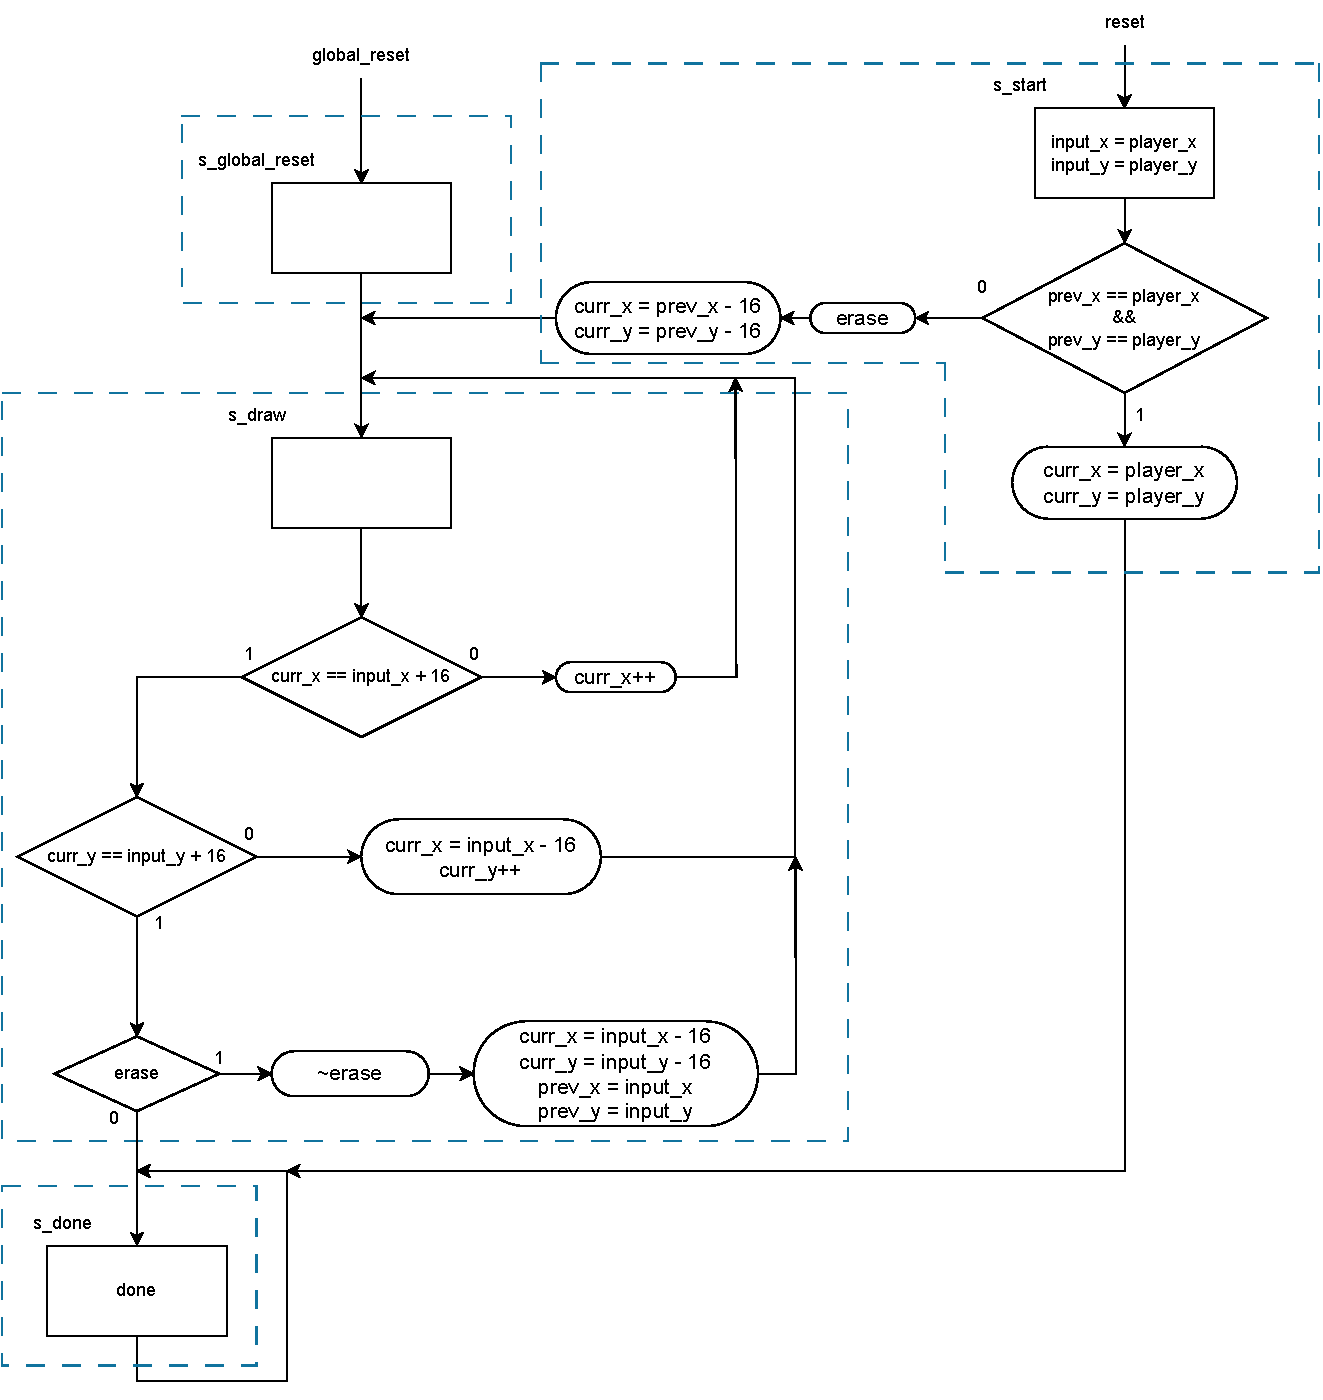
\includegraphics[scale = 0.57]{Images/Player Drawer.pdf}
                \caption{Player Drawer ASM chart}
            \end{figure}
            There is also a system responsible for tracking and updating the values of the player's location with the input of the N8 controller. The player drawer begins from a reset of the state machine that sets new values for the input into the module. The module then compares the values received on the system reset to the values that were last in the system. In the case that they are the same values as previous, the state machine moves into the done state to signify that no values should be updated since last iteration. In the case that they are not the same as the last iteration, the state machine sets the erase signal to high and updates the current values to be 16 less than they were previously, this ensures that the state will be updated on the next cycle, and then moves into the draw state The draw state then continues to iterate through, updating the current values of x and y until they are equal to the proper input. Finally the erase signal is turned off and the proper value is set for the player to be drawn on the next cycle. The machine then enters the done state and finishes.

        \subsection{Top Level Module}
            \begin{figure}[H]
                \centering
                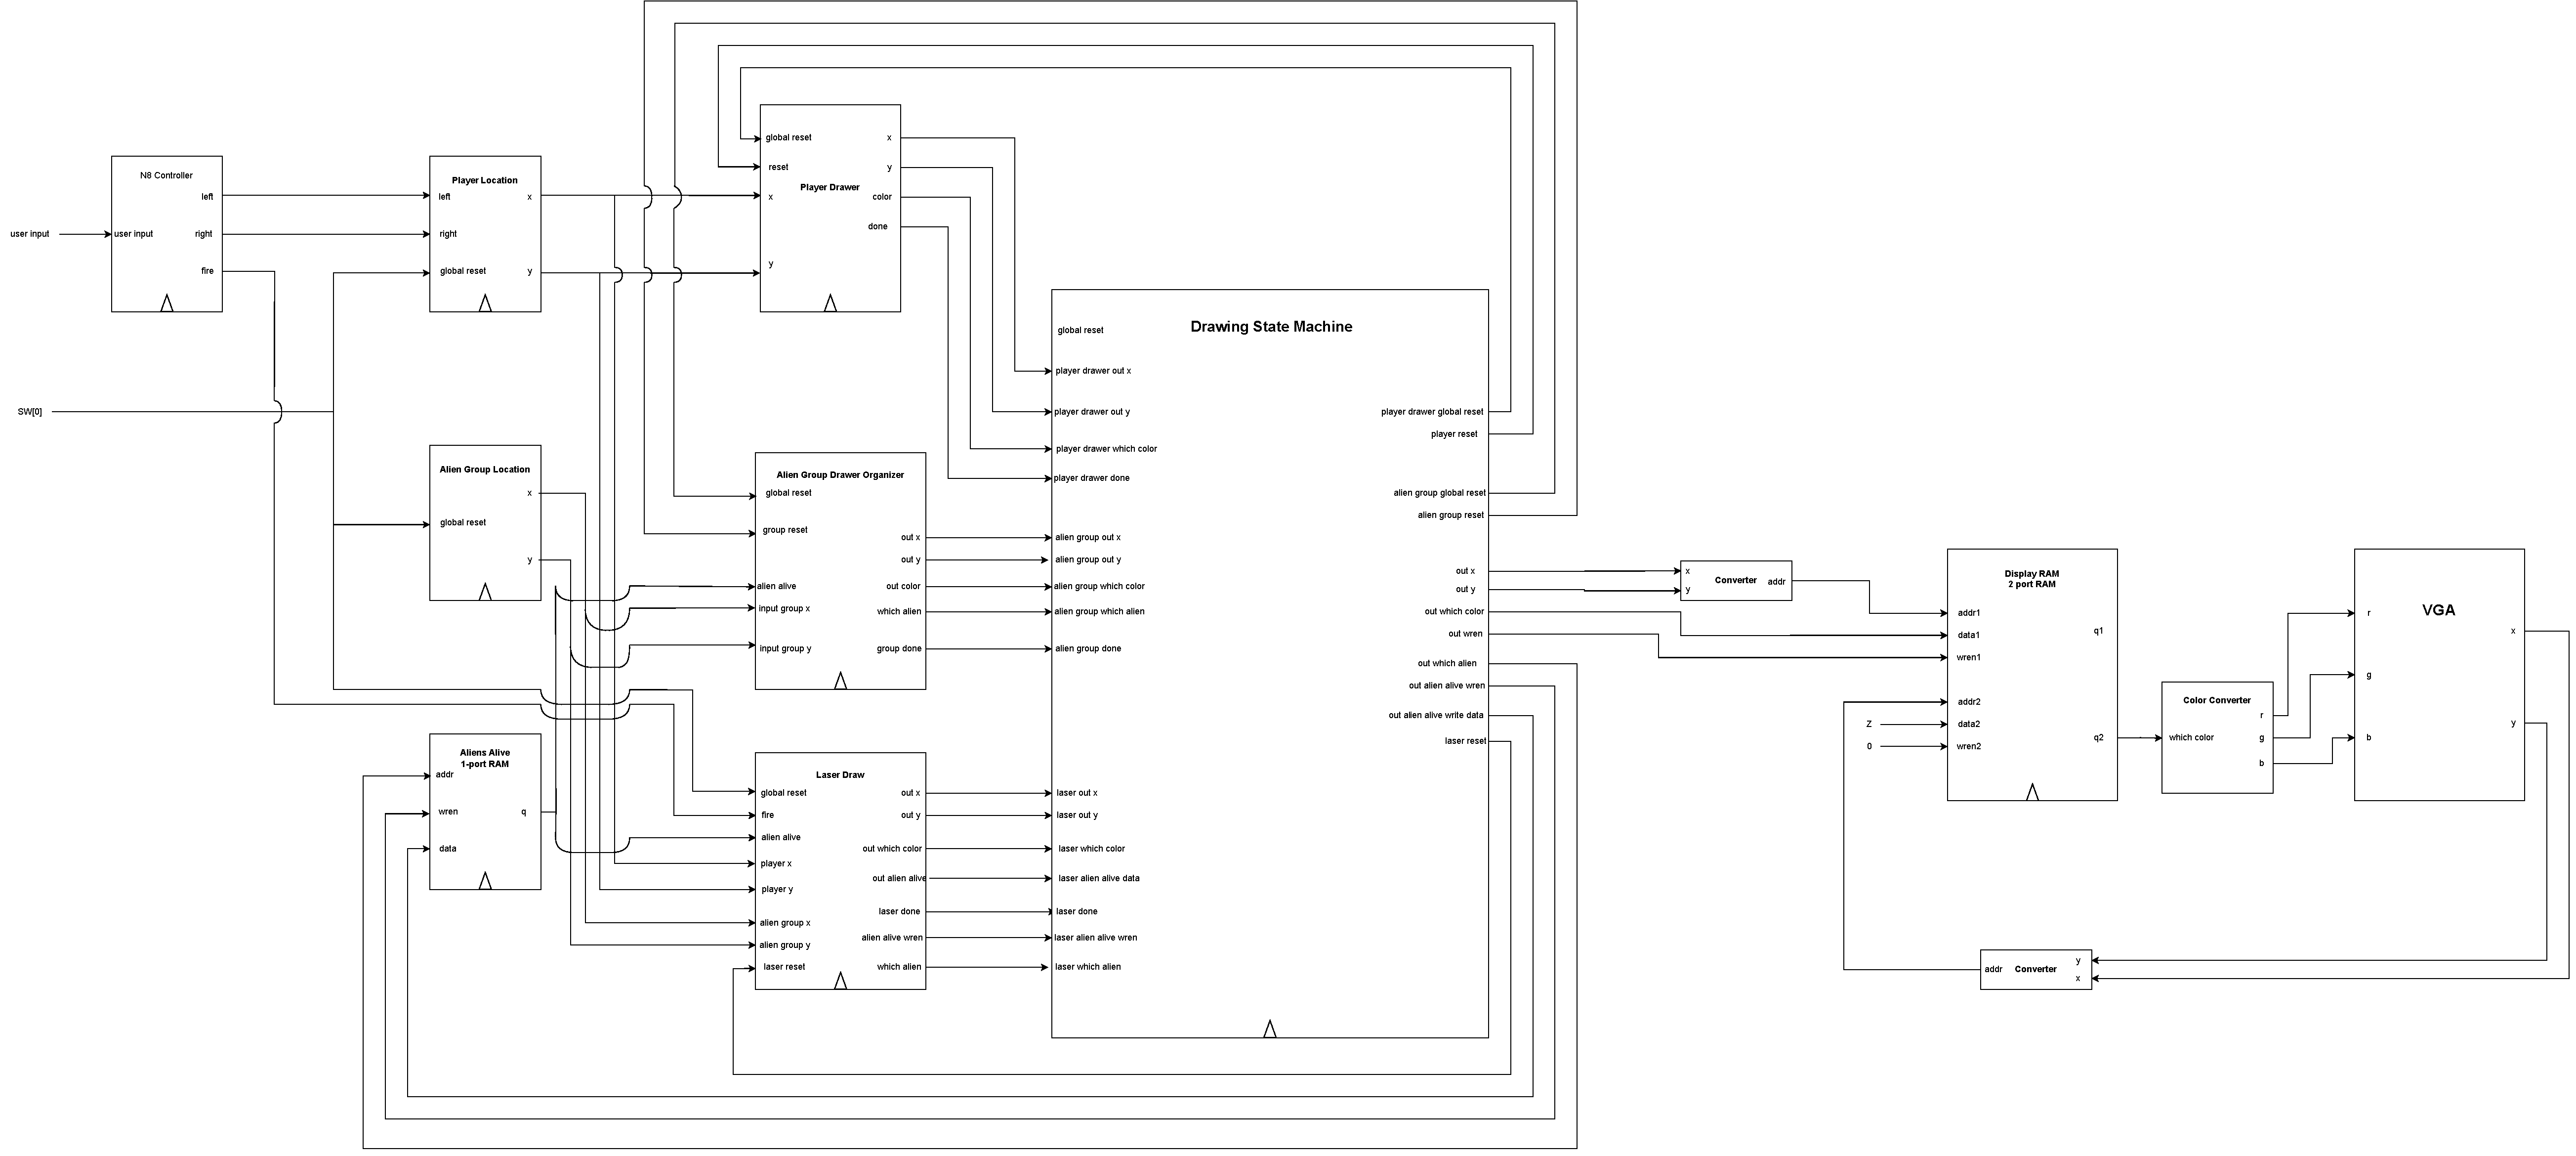
\includegraphics[scale = 0.17]{Images/Top Level Module Block Diagram.pdf}
                \caption{Top Level Block Diagram}
            \end{figure}

    \section{Results}
    The system we implemented in the lab was a game similar to Space Invaders. The N8 controller allowed the user to be able to control the player's movement and laser gun. Other modules were made to simulate the aliens and their behavior within the game. The modules consist of many algorithmic state machines that are tasked with updating the location of the players, aliens, and laser blasts based on the current conditions of the game. Finally, there is a drawer that cycles through drawing the updated pieces to the VGA display.

        \subsection{Color Converter Module}
            \begin{figure}[H]
                \centering
                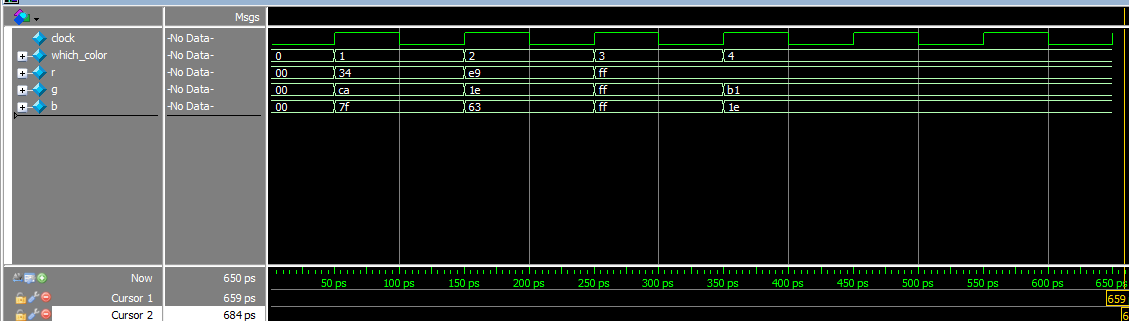
\includegraphics[scale = 0.53]{Images/Testbench Color Converter .png}
                \caption{Color Converter Testbench}
            \end{figure}
            The color converter has ``which\_color'' as an input and outputs the RGG values which correspond to that color. This testbench shows that the color converter module correctly converts from the number of the color to the RGB value of the color we want.

        \subsection{Player Location Module}
            \begin{figure}[H]
                \centering
                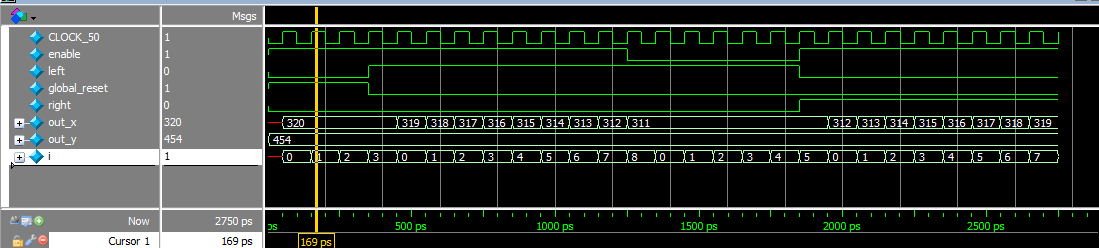
\includegraphics[scale = 0.53]{Images/Testbench Player Location.png}
                \caption{Player Location Testbench}
            \end{figure}
            This module takes the clock, enable, left, right, and global reset as input signals. It outputs the x and y value of the location of the center of the player's spaceship. The testbench shows that upon global reset, the x and y values are reset to the starting location on the screen. It shows that when enable is high, the x value is decremented when left is high and is incremented when right is high. It also constrains the x value so that the player does not reach the edge of the screen.

        \subsection{Alien Group Location}
            \begin{figure}[H]
                \centering
                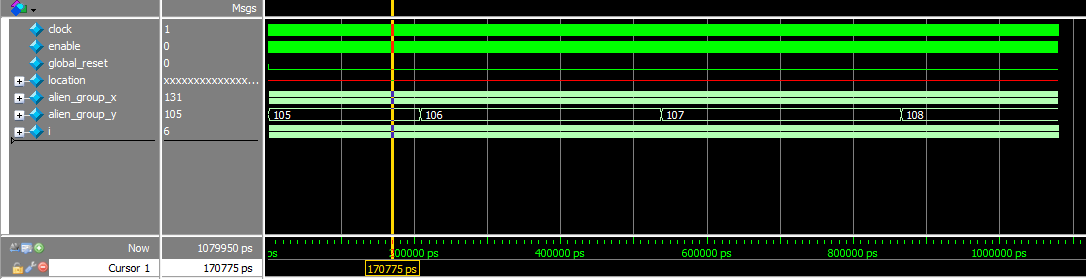
\includegraphics[scale = 0.53]{Images/Testbench Alien Group Location.png}
                \caption{Alien Group Location Testbench}
            \end{figure}
            This module takes the clock, enable, and global reset as input signals. It outputs the x and y values of the center of the group of aliens. The module is essentially a 2D counter. Initially the aliens move to the left, so after the global reset the x value starts decrementing. Once the x value reaches the value where the left most aliens are close to touching the edge of the screen, the y value is incremented and the x values start incrementing until the group reaches the right side of the screen. Then the process repeats. The testbench shows that the y value is incremented and the x value increment/decrement direction changes when the group hits the edge of screen.
        \subsection{Drawing State Machine Module}
            \begin{figure}[H]
                \centering
                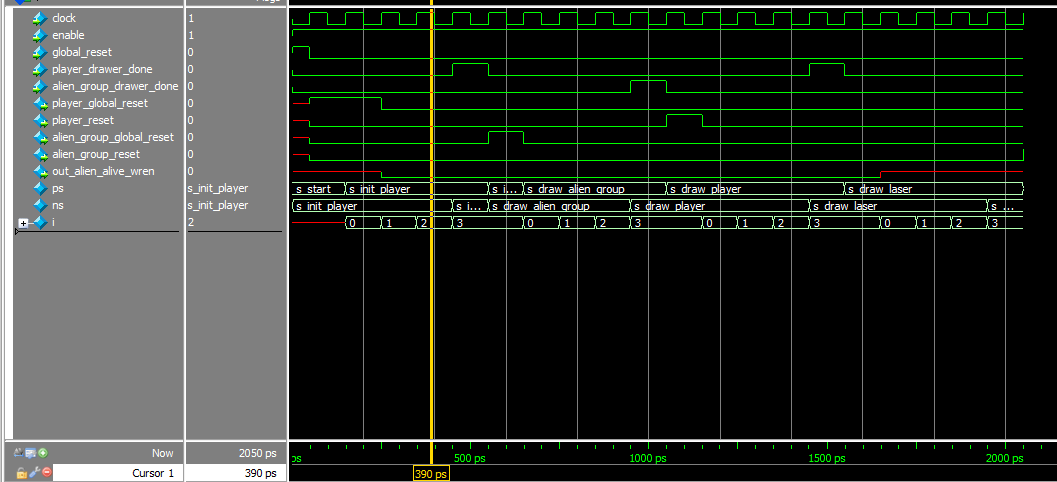
\includegraphics[scale = 0.53]{Images/Testbench Drawing State Machine.png}
                \caption{Drawing State Machine Testbench}
            \end{figure}
            The drawing state machine module is in charge of handling what gets drawn and in which order. For every new frame the drawing state machine first draws the player, then the laser (if it exists), and then the group of aliens. The test bench shows that the module correctly initially draws the player, and then once the player is finished, switches to drawing the group of aliens, and then once the group of aliens is done, draws the laser, then the group of aliens, then the player and then the cycle repeats. This testbench shows that the machine correctly switches states when it sees that the player, alien group, and laser are finished drawing.

        \subsection{Alien Group Drawer}
            \begin{figure}[H]
                \centering
                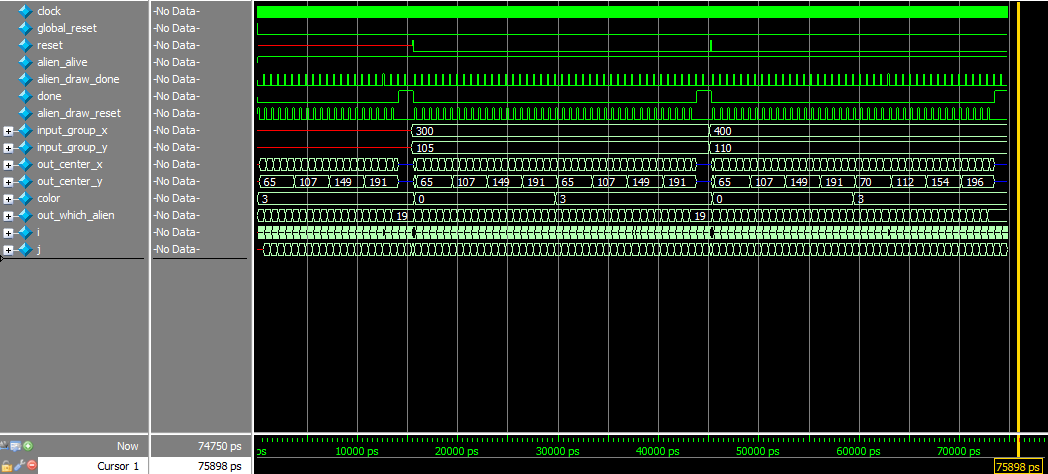
\includegraphics[scale = 0.53]{Images/Testbench Alien Group Drawer.png}
                \caption{Alien Group Drawer Testbench}
            \end{figure}
            This testbench manages drawing the aliens. It goes through each alien, if its alive, then it will draw it. It takes the clock, a global reset, a reset, input data from alien alive RAM, alien draw done, and the location of the group of aliens. This testbench shows that the module correctly cycles through all 20 of the aliens and correctly outputs the reset signal when an alien needs to be drawn, and moves on to the next alien when that alien has finished drawing.
        \subsection{Alien Drawer}
            \begin{figure}[H]
                \centering
                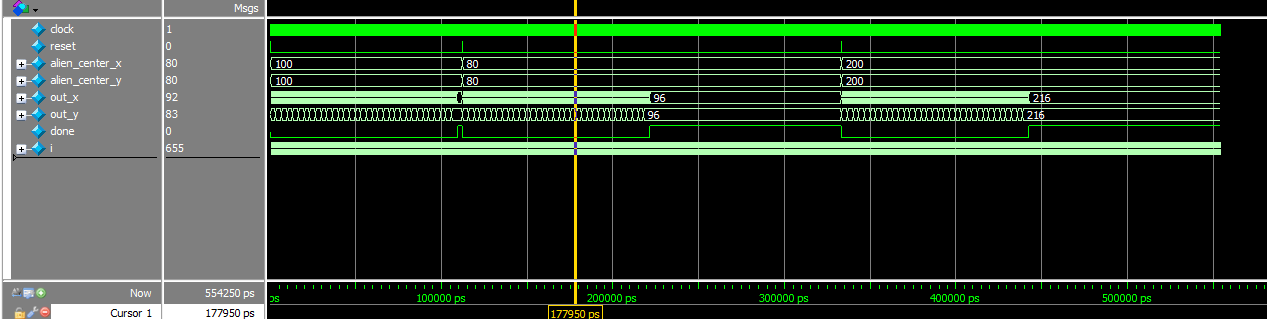
\includegraphics[scale = 0.49]{Images/Testbench Alien Drawer.png}
                \caption{Alien Drawer Testbench}
            \end{figure}
            This module takes the clock, reset, and the center of the alien that is going to be drawn as inputs. It outputs the xy coordinate of a pixel that needs to be colored and outputs done when the alien has finished drawing. The testbench shows that the module correctly starts when the reset signal is high. The testbench then shows that the module ``draws'' the rectangle of the pixels that make up of the alien. It then shows that the done signal is high once the module has finished drawing one alien.
        \subsection{Player Drawer}
            \begin{figure}[H]
                \centering
                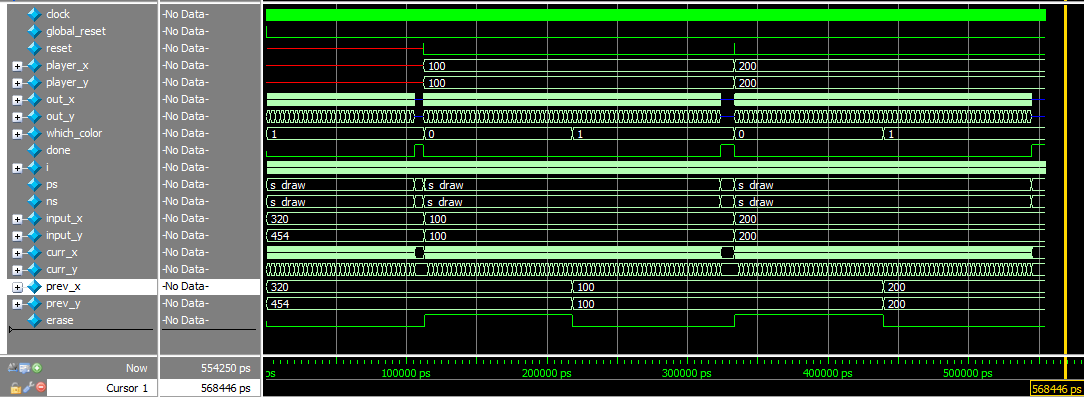
\includegraphics[scale = 0.53]{Images/Testbench Player Drawer.png}
                \caption{Player Drawer Testbench}
            \end{figure}
            This module draws the player. So, it takes the clock, global reset, reset, and the XY coordinates of the player as inputs. It then outputs the XY coordines of a pixel, the color that pixel should be, and whether the module is done drawing the player for this frame. The test bench shows that the player is drawn initially when the global reset signal is high. It also shows that when the player XY coordinate changes and the reset signal is high, the module ``erases'' the drawing from the previous frame and redraws the player at its new location. It also shows that the output which\_color and done corerctly match the stage of the machine.

        \subsection{Top Level}
            \begin{figure}[H]
                \centering
                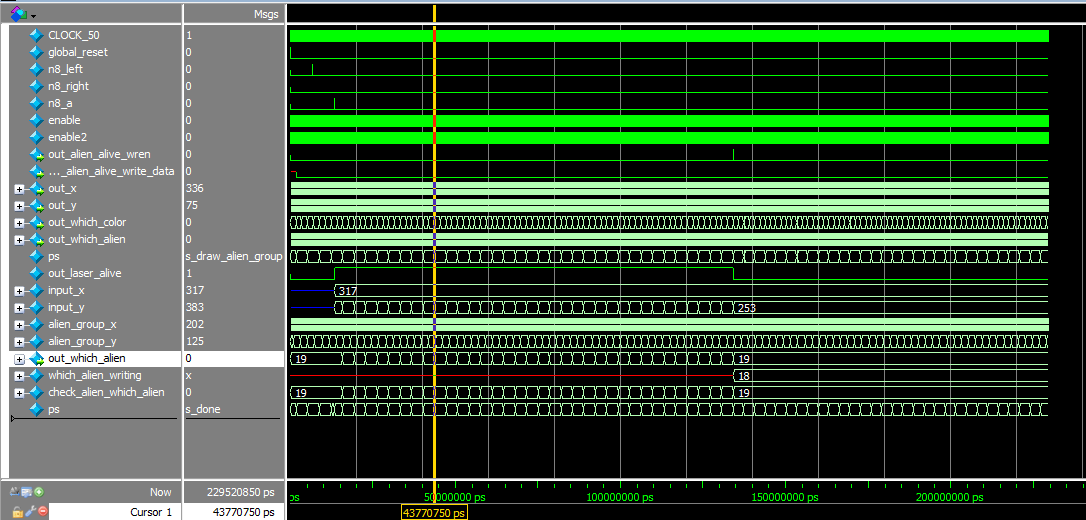
\includegraphics[scale = 0.53]{Images/Testbench Top Level.png}
                \caption{Top Level Testbench}
            \end{figure}
            This testbench is as close to a top level test bench as we could get. Since it is very complicated to simulate the N8 controllers and VGA driver, those are the only things that were left out of the testbench module. This test bench shows that the game correctly starts on the global reset signal. It demonstrates the drawing state machine going through all it states, the player moving to the left, and the player firing a laser. Once that laser hits an alien, the laser and the alien ``die'' and the alien alive RAM get written to. This testbench showed that all the connections between the lower level modules are correct. There is no logic at this level. `'

        \newpage
        \subsection{Flow Summary}
            Fitter Status : Successful - Thu Dec  7 23:12:26 2023 \\
            Quartus Prime Version : 17.1.0 Build 590 10/25/2017 SJ Lite Edition \\
            Revision Name : DE1\_SoC1 \\
            Top-level Entity Name : DE1\_SoC1 \\
            Family : Cyclone V \\
            Device : 5CSEMA5F31C6 \\
            Timing Models : Final \\
            Logic utilization (in ALMs) : 905 / 32,070 ( 3 \% ) \\
            Total registers : 637 \\
            Total pins : 118 / 457 ( 26 \% ) \\
            Total virtual pins : 0 \\
            Total block memory bits : 1,228,820 / 4,065,280 ( 30 \% ) \\
            Total RAM Blocks : 151 / 397 ( 38 \% ) \\
            Total DSP Blocks : 5 / 87 ( 6 \% ) \\
            Total HSSI RX PCSs : 0 \\
            Total HSSI PMA RX Deserializers : 0 \\
            Total HSSI TX PCSs : 0 \\
            Total HSSI PMA TX Serializers : 0 \\
            Total PLLs : 1 / 6 ( 17 \% ) \\
            Total DLLs : 0 / 4 ( 0 \% ) \\

            Analysis \& Synthesis Status : Successful - Thu Dec  7 23:11:37 2023 \\
            Quartus Prime Version : 17.1.0 Build 590 10/25/2017 SJ Lite Edition \\
            Revision Name : DE1\_SoC1 \\
            Top-level Entity Name : DE1\_SoC3 \\
            Family : Cyclone V \\
            Logic utilization (in ALMs) : N/A \\
            Total registers : 588 \\
            Total pins : 118 \\
            Total virtual pins : 0 \\
            Total block memory bits : 1,228,820 \\
            Total DSP Blocks : 5 \\
            Total HSSI RX PCSs : 0 \\
            Total HSSI PMA RX Deserializers : 0 \\
            Total HSSI TX PCSs : 0 \\
            Total HSSI PMA TX Serializers : 0 \\
            Total PLLs : 1 \\
            Total DLLs : 0 \\
            
    \newpage
    \section{Experience Report}
        This lab was much harder than all the others. The hardest part about all of this was probably having to erase the previous frame's drawings. That significantly complicated stuff. Also managing which module was writing to the RAM at what time was hard. We also sigfnificantly underestimated how much work Space Invaders is. \\

        This lab took approximately 66 hours, broken down as follows:
        \begin{description}
            \item[Design, Coding \& Debugging:] 51 hours
            \item[Write up:] 15 hours
        \end{description}   
        
\end{document}
